\subsection{Résumés de textes}

La synthèse de textes est un domaine qui se développe et qui est de plus en plus utilisé.
On peut noter, par exemple, l'apparition d'outils gratuits en ligne permettant de synthétiser des textes, par exemple <<~resoomer~>>, ou <<~autosummarizer~>>.
Il existe aussi des applications mobiles permettant de résumer des articles d'actualité, avec <<~inshorts~>>.
Synthétiser des textes automatiquement est utile et peut faire gagner énormément de temps à une personne et même à des compagnies dans leur globalité si les outils de synthèse utilisés sont performants et produisent des résumés entraînant le moins de perte d'information possible.

Pour tirer parti des méthodes de synthèses de textes d'un point de vue global sur une compagnie, on peut imaginer la mise en place d'un outil de synthèse accessible à tout moment au sein de l'ERP de l'entreprise.

Il y a trois types de synthèse possible~:~
\\
\begin{itemize}
    \item[\tiny$\bullet$] La synthèse par extraction extrait les phrases jugées les plus importantes du texte et les concatène pour produire un résumé.
    Cette méthode est très utilisée dans les systèmes réels.
    
    \item[\tiny$\bullet$] La synthèse par abstraction vise à résumer un texte en générant de nouvelles phrases à partir des informations importantes comprises dans le texte initial.
    Cette méthode permet de générer des résumés intelligents qui reprennent les informations utiles du texte dans sa globalité.
    Elle est peu mise en place dans les systèmes réels, de par sa complexité.
    
    \item[\tiny$\bullet$] La synthèse par compression de phrases consiste en la suppression des mots jugés superflus au sein des phrases.
    Elle peut aussi éliminer des phrases complètes si celles-ci ne sont pas jugées utiles.
\end{itemize}
~\\

De nombreux outils utilisant la synthèse par extraction, parfois liée à la compression de phrases, existent sur internet.
L'intérêt d'ajouter un outil réalisant la même tâche au sein d'un ERP a donc très peu d'intérêt.
Cependant, la synthèse par abstraction permet des résumés de bien meilleure qualité et il serait donc utile de mettre un tel outil à disposition des employés.

Lorsqu'il s'agit de traiter des problèmes concernant le traitement automatique du langage naturel, les modèles d'apprentissage profond généralement utilisés sont les RNN (<<~Recurrent Neural Network~>>, <<~réseaux de neurones récurrents~>>).
Les RNN sont un type de réseaux de neurones qui possède un cycle dans sa structure neuronale et qui sont capables de gérer des données d'entrées de taille variables et notamment des séquences.
Dans le cadre du traitement du langage naturel, les phrases correspondent à des suites de caractères, qui peuvent être considérées par un RNN comme des séquences.

Les RNN seuls ont beaucoup été utilisés dans la recherche sur le traitement du langage, mais des employés de \textsc{Google} ont développé un nouveau modèle en 2014, le <<~sequence to sequence model~>> \cite{seq2seq}, modèle de séquence à séquence.
Ce modèle est composé de deux parties qui se complètent~:~la première est un encodeur, la seconde est un décodeur.
Il s'agit de deux RNN différents qui sont combinés pour n'en former qu'un seul.

Le principe est le suivant~:~le rôle de l'encodeur est de comprendre la séquence donnée en entrée et de créer une représentation abstraite de celle-ci.
C'est comparable à un être humain qui comprend une phrase, celle-ci est représentée au sein du cerveau de manière abstraite, en tant que pensée, ce qui permet à ce dernier de la traiter plus facilement.

Cette représentation abstraite est ensuite donnée en entrée au décodeur, celui-ci va créer une nouvelle séquence correspondante aux données d'entrées.
Le fonctionnement est schématisé ci-dessous.

\FloatBarrier
\begin{figure}[h!]
    \begin{center}
        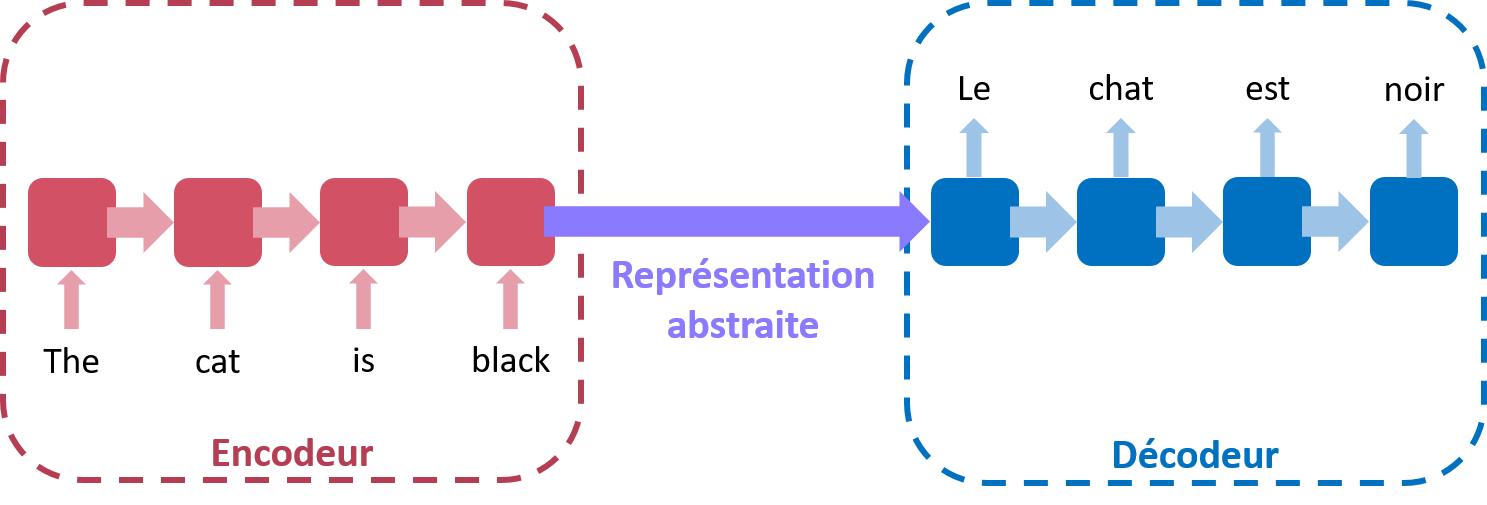
\includegraphics[width = 0.9\textwidth]{seq2seq}
    \end{center}
    \caption{Fonctionnement schématique d'un modèle de séquence à séquence}
    \label{figure:seq2seq}
\end{figure}
\FloatBarrier

Ce type de modèle a permis d'accélérer grandement la recherche dans le traitement du langage naturel et peut notamment être utilisé pour la synthèse de texte.
Correctement entraîné, un modèle de ce type est capable de comprendre les informations d'un texte qui ont une grande importance afin de les extraire grâce à l'encodeur.
Le décodeur est ensuite capable d'utiliser ces données importantes pour recréer des phrases dans un langage correct et compréhensible.
Le même modèle peut aussi être entraîné pour de la traduction automatique, par exemple.

Le principal problème que l'on pourrait rencontrer en développant un tel modèle est que son entraînement demande une grosse puissance de calcul.
Il faut donc une excellente machine pour effectuer l'entraînement de ce modèle.
En revanche, son utilisation demande peu de ressources, les machines des utilisateurs n'ont donc pas besoin d'être très performantes.